\documentclass{beamer}
\usepackage[utf8]{inputenc}
\usepackage[portuguese]{babel}
\usepackage{upgreek}
\usepackage{amsmath}
\usepackage{amsthm}
\usepackage{amsfonts}
\usepackage{wasysym}
\usepackage{amssymb}
\usepackage{amsthm}
\usepackage{calligra}
\usepackage{calrsfs}
\usepackage[mathscr]{euscript}
\usepackage{graphicx}
\usepackage{tikz-cd}
\usepackage{verbatim}
\usetikzlibrary{positioning}
\newcommand{\negrito}[1]{\mbox{\boldmath{$#1$}}}
\usepackage{ragged2e}%justifying

\usetheme{Warsaw}


    \definecolor{myblue1}{RGB}{214, 26, 26}%Vermelho
    \definecolor{myblue2}{RGB}{247, 120, 0}%Laranja
    \definecolor{myblue3}{RGB}{214, 26, 26}
    \definecolor{myblue4}{RGB}{26,89,142}

    \setbeamercolor*{structure}{fg=myblue1,bg=blue}
    \setbeamercolor*{palette primary}{use=structure,fg=white,bg=structure.fg}
    \setbeamercolor*{palette secondary}{use=structure,fg=white,bg=structure.fg!75!black}
    \setbeamercolor*{palette tertiary}{use=structure,fg=white,bg=structure.fg!50!black}
    \setbeamercolor*{palette quaternary}{fg=black,bg=white}

    \setbeamercolor*{item projected}{fg=red,bg=myblue3!80}
    \setbeamercolor*{block title example}{fg=white,bg=myblue4}
    \setbeamercolor*{frametitle}{fg=black}

    \setbeamertemplate{blocks}[rounded][shadow=true]

    \makeatletter
    
    \pgfdeclarehorizontalshading[frametitle.bg,frametitle right.bg]{beamer@frametitleshade}{\paperheight}{%
      color(0pt)=(myblue2);
      color(\paperwidth)=(white)}

    \defbeamertemplate*{footline}{mysplit theme}
    {%
      \leavevmode%
      \hbox{\begin{beamercolorbox}[wd=.5\paperwidth,ht=2.5ex,dp=1.125ex,leftskip=.3cm plus1fill,rightskip=.3cm]{author in head/foot}%
        \usebeamerfont{author in head/foot}\insertshortauthor
      \end{beamercolorbox}%
      \begin{beamercolorbox}[wd=.5\paperwidth,ht=2.5ex,dp=1.125ex,leftskip=.3cm,rightskip=.3cm plus1fil]{title in head/foot}%
        \usebeamerfont{title in head/foot}\insertshorttitle\hfill
        \insertframenumber/\inserttotalframenumber\hspace*{0.5em}
      \end{beamercolorbox}}%
      \vskip0pt%
    }
\theoremstyle{plain}
\newtheorem{thm}{Theorem}[section] % reset theorem numbering for each chapter

\theoremstyle{definition}
\newtheorem{definicao}[thm]{Definição}

\theoremstyle{definition}
\newtheorem{exemplo}[thm]{Exemplo}

\theoremstyle{definition}
\newtheorem{contraexemplo}[thm]{Contraexemplo}

\theoremstyle{definition}
\newtheorem{corolario}[thm]{Corolário}

\theoremstyle{definition}
\newtheorem{teorema}[thm]{Teorema}

\theoremstyle{definition}
\newtheorem{proposicao}[thm]{Proposição}

\theoremstyle{definition}
\newtheorem{lema}[thm]{Lema}

\theoremstyle{definition}
\newtheorem{observacao}[thm]{Observação}

\usepackage{commath}
\DeclareSymbolFont{extraup}{U}{zavm}{m}{n}
\DeclareMathSymbol{\varheart}{\mathalpha}{extraup}{86}
\DeclareMathSymbol{\vardiamond}{\mathalpha}{extraup}{87}
\newcommand{\heart}{\ensuremath\heartsuit}
\newcommand{\diamonde}{\ensuremath\diamondsuit}

\title[]{O Cálculo Variacional e sua importância para a Relatividade Geral}
%\subtitle[]{I ERMAC-MS}

\author[Sacha Ferreira, Douglas Smigly, Daniel Kawai, José de Araújo]{
Sacha Lucien Moser Ferreira \inst{1} 
\newline Douglas de Araujo Smigly \inst{2}
\newline  Daniel Eiti Nishida Kawai \inst{3}
\newline José Carlos Neves de Araujo \inst{4} \vspace{-6pt}
}
\institute[UNESP, USP, INPE]{
 \inst{1} Instituto de Biociências, Letras e Ciências Exatas, UNESP \and 
\inst{2} Instituto de Matemática e Estatística, USP \and 
\inst{3} Instituto de Matemática e Estatística, USP \and 
\inst{4} Instituto Nacional de Pesquisas Espaciais, INPE \vspace{-6pt}
}
\date{I ERMAC-MS, setembro de 2020}

\begin{document}

\frame{\maketitle}

\begin{frame}{Agradecimentos}
    %Do Sacha
    Agradecemos a
\begin{itemize}
\item Odilon Otávio Luciano (IME-USP);
    \item Beatriz Nahas Pinto;
    \item Antônio Silva Neto (IPRJ);
\item Sandra Malta (LNCC);
\item Geraldo Nunes (IBILCE-UNESP);
\item Berenice Camargo Damasceno (UNESP ILHA);
\item José Carlos Neves de Araújo (INPE)
\item Luciano Barbanti (\textit{in memoriam}) (UNESP ILHA);
\item Antonio Fazoli (\textit{in memoriam}) (COLÉGIO OBJETIVO INTEGRADO);
\item Zé Carlos (INPE-SJC)
\end{itemize}

\end{frame}
\begin{frame}{Introdução}
    %Problemas de otimização possuem uma grande importância para diversas áreas da Física, Matemática, Engenharia, Biologia, Economia e Química.
    O problema principal do Cálculo Variacional está relacionado a seguinte questão:
    
    \begin{block}{O problema do Cálculo Variacional}
    Dados $x_1$ e $x_2,$ queremos encontrar uma função $y(x)$ que possui valores fixos nesses pontos e cuja integral de linha (integral calculada ao longo da curva) 
\[
J = \int\limits_{x_1}^{x_2} f\left(y, \od{y}{x}, x\right) \dif x\]
seja um ponto crítico, isto é, que é um ponto no domínio da função onde a primeira derivada é nula. 
\end{block}

Em outras palavras, o objetivo é encontrar $y(x)$ com pontos fixos $y_1 = f(x_1)$ e $y_2 = f(x_2)$ tal que a integral $J$ seja estacionária.

\end{frame}


\begin{frame}{O problema da Geodésica}
    Em espaços planos, as geodésicas são definidas habitualmente como o menor caminho entre dois pontos.
    
    \begin{block}{Geodésica}
    Seja $M \subset \mathbb{R}^n$ uma subvariedade de dimensão $k$. Dados dois pontos $p_1$ e $p_2 \in M$, a curva $\gamma:[a, b] \rightarrow M$ regular de classe $\mathcal{C}^1$ que os conecta, ou seja, que satisfaça $\gamma(a) = p_1$ e $\gamma(b) = p_2$, e também tenha comprimento mínimo, é chamada de geodésica.
    \end{block}
    \begin{figure}[!h]
\begin{center}
%\caption{Deflação da luz devido a massa do Sol.} \label{fig:02}
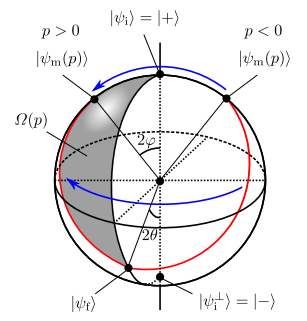
\includegraphics[width=0.35\textwidth]{Template_ERMACMS/bloch.png}l
\end{center}
\end{figure}
\end{frame}


\begin{frame}
\frametitle{O problema da Geodésica}

Supondo que $x^\mu = x^\mu(s)$ e tomando $p^\mu = \frac{dx^\mu}{ds}$ tangente à curva e a Lagrangiana sendo escrita na
forma~$\mathcal{L} = g_{\mu \upnu} p^\mu p^\upnu$, então temos que equações de
Euler-Lagrange e geodésicas são dadas respectivamente por
$$
\frac{d}{ds}\frac{\partial \mathcal{L}}{\partial p^\lambda} = \frac{\partial\mathcal{L}}{\partial x^\lambda} = 0
$$
e
$$
\frac{d^2 x^\rho}{ds^2} + \Upgamma^\rho_{\mu \upnu}\frac{dx^\mu}{ds}  \frac{dx^\upnu}{ds} =0
$$
\end{frame}

\begin{frame}{Deflação da luz}
\justifying
    As geodésicas de Schwarzschild descrevem o movimento de partículas de massa infinitesimal no campo gravitacional de uma massa central fixa, e são responsáveis pelas previsões precisas da precessão anômala dos planetas no Sistema Solar e o fenômeno de deflexão da luz pela gravidade.

\begin{figure}[!h]
\begin{center}
\caption{Deflação da luz devido a massa do Sol.} \label{fig:02}
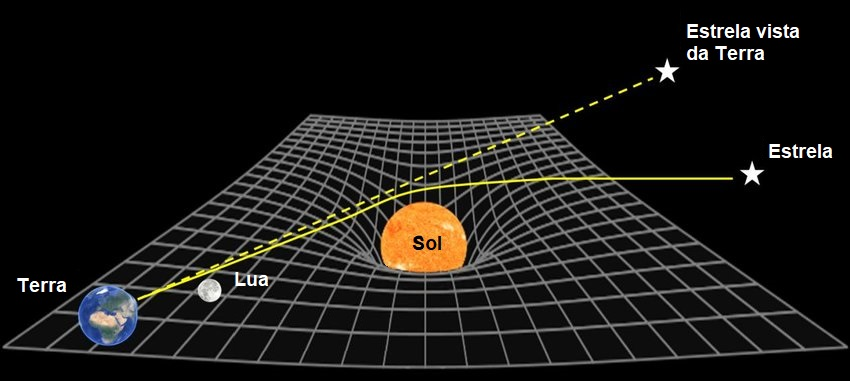
\includegraphics[width=0.85\textwidth]{Template_ERMACMS/defle.png}
\end{center}
\end{figure}
\end{frame}

\begin{comment}

\begin{frame}
Tais geodésicas provém da métrica de Schwarzchild. A equação da órbita de uma partícula será
\[
\left( \frac{\dif r}{\dif \varphi} \right)^{2} = \frac{r^{4}}{b^{2}} - \left( 1 - \frac{2m}{r} \right) \left( \frac{r^{4}}{a^{2}} + r^{2} \right),
\]
cuja solução é 
\begin{equation}\label{Orb}
\varphi = \displaystyle\int \dfrac{1}{\pm r^{2} \sqrt{\dfrac{1}{b^{2}} - \left( 1 - \dfrac{2m}{r} \right) \left( \dfrac{1}{a^{2}} + \dfrac{1}{r^{2}} \right)}}\dif r,
\end{equation}
onde tomamos $a = \frac{h}{c}$ e $b = \frac{cL}{E},$ no qual $h$ é o momento angular específico, $c$ é a velocidade da luz, $L$ é o momento angular e $E$ é a energia total. 
\end{frame}
\end{comment}

\begin{frame}{Equações de Campo da Relatividade Geral}
    As equações de campo são expressões dinâmicas que descrevem a maneira como matéria e energia modificam a geometria do espaço-tempo.
    \begin{block}{Equações de campo}
    As equações de campo de Einstein que sintetizam a interação da matéria com a geometria do espaço-tempo são dadas por
\[R_{\mu \nu} - \tfrac{1}{2}R g_{\mu \nu} = \frac{8 \pi G }{c^4} T_{\mu \nu},\]
onde $R_{\mu \nu}$ é o tensor de curvatura de Ricci, $R$ é a curvatura escalar, $ g_{\mu \nu}$ é o tensor métrico, $G$ é a constante universal da gravitação de Newton, $c$ é a velocidade da luz no vácuo e $T_{\mu \nu}$ é o tensor energia-momento.
\end{block}

%Convém salientar que a métrica de Schwarzchild dada em \ref{Sch} é uma solução exata para as equações de campo da Relatividade Geral. 
\end{frame}

\begin{frame}{Equações de Campo da Relatividade Geral}
\justifying
Até então nos tornamos nossa atenção para equações de campo no vacuo.
Para obter a equação completa, assumiremos que existem outros campos
presentes além do campo gravitacional, que pode ser descrito por
uma densidade Lagragiana apropriada $\mathcal{L}_M$. Então a ação é
$$
I = \int_\Omega (\mathcal{L}_G + \kappa\mathcal{L}_M)d\Omega
$$
Ambas as Lagrangianas são funcionais da métrica e sua derivadas,
variando com respeito a $g_{ab}$, obtemos
$$
\frac{\delta \mathcal{L}_M}{\delta g_{ab}} = (-g)^{\frac{1}{2}}T^{ab}
$$
\end{frame}

\begin{frame}{Ação de Hilbert-Einstein}
\justifying
    A formulação variacional permite um melhor entendimento físico da fonte de campo gravitacional e uma maneira mais fácil de englobar outros campos na teoria, ou ainda formular teorias alternativas à Relatividade Geral.
    A partir do funcional ação dado por \[\mathcal{S} = \int\limits_{\Omega} \mathcal{L} d^4 x,\] onde $d^4x$ é o elemento de 4-volume, o princípio da mínima ação nos diz que $\delta S = 0,$ de onde pode-se obter
 \[
 S= - {1 \over 2\kappa}\int R \sqrt{-g} d^4x,
 \]
 conhecida como \textit{ação de Hilbert-Einstein}. Fazendo $\delta S = 0$, como já mencionado, obtemos as equações de campo da Relatividade Geral.
\end{frame}
%\begin{frame}{Conclusão}
%    Podemos concluir que a conclusão foi concluída.
%\end{frame}
\begin{frame}{Conclusão}
\justifying
O operador de Lagrange ajuda a inferir as equações de Euler-Lagrange a partir da minimalização do comprimento, de modo que podemos retratar de maneira mais prática o comportamento de partículas diante da ação da gravidade sobre o espaço-tempo.

A ação de Hilbert-Einstein nos ampara na incumbência de robustecer uma dedução concisa das equações de campo de Einstein e descrever o comportamento de grandezas físicas.

Em suma, o cálculo variacional permite converter problemas de otimização em equações diferenciais parciais, fornecendo uma simplificação determinante para que os problemas sejam analisados sobre um escopo diferente que se torna aquiescente com a abordagem desejada para a resolução desses problemas. %é mais fácil de lidar com estas.

\end{frame}

\begin{frame}{Conclusão}
\[
\textbf{Obrigado!}
\]
\center
 Agradecemos a Comissão Organizadora do I ERMAC-MS e a SBMAC pela oportunidade e pela organização do evento!

\end{frame}


\begin{frame}
\begin{thebibliography}{99} 
\frametitle{Bibliografia}

\bibitem{Castro}
CASTRO, L. M. {\bf O Cálculo Variacional e as Curvas Cicloidais}. Dissertação de Mestrado. Universidade de Brasília, 2014.

\bibitem{CHANDRASEKHAR}
CHANDRASEKHAR, S. {\bf On the derivation of Einstein’s field
equations}, American Journal of Physics,v. 40, n. 2, p. 224–234, 1972.

\bibitem{CHAKRABORTY}
CHAKRABORTY, S. {\bf Boundary terms of the Einstein-Hilbert action
}, Fundamental Theories of Physics, 187, p. 43–59, 2017.

\bibitem{Einstein} 
D'INVERNO, R. {\bf Introducing Einstein's Relativity}. Clarendon Press, 1992.

\end{thebibliography}
\end{frame}

\begin{frame}
\begin{thebibliography}{99} 
\frametitle{Bibliografia}
\bibitem{Odzijewicz} 
ODZIJEWICZ, T.; MALINOWSKA, A. B.; TORRES, D. M. T. {\bf Fractional Variational Calculus with Classical and Combined Caputo Derivatives}. Nonlinear Analysis, v. 75, n.3, p. 1507--1515, 2012.
\bibitem{Paolozzi} 
PAOLOZZI A.; PARIS C.; SINDONI G; and TARTAGLIA, A. {\bf The LARES Mission: An Opportunity to Teach General Relativity - Frame Dragging and Lense-Thirring Effect}. In: Proceedings of the 7th International Conference on Computer Supported Education. p. 343--348, 2015

\bibitem{Riewe} 
RIEWE, F. {\bf Mechanics with fractional derivatives} Physics Review, v. 55, n. 1, p. 3581--3592, 1997.


\bibitem{Tamate}
TAMATE, S.; NAKANISHI, T.; KOBAYASHI, H.; KITANO, M. {\bf Geometrical aspects of weak measurements and quantum erasers}, New Journal of Physics, v. 11, n. 9, 2009.

\end{thebibliography}
\end{frame}

\begin{frame}
\begin{thebibliography}{99}
\frametitle{Bibliografia}

\bibitem{Tausk}
TAUSK, D. V. {\bf Notas de aula de Cálculo Variacional}, {\it Minicurso IF-Instituto de Fisica 2019}, Universidade de São Paulo, 2019.

\bibitem{Will}
WILL, C. M. {\bf The Confrontation between General Relativity and Experiment}, Living Reviews in Relativity, v. 17, n. 4, 2014.

\bibitem{Khuri}
KHURI, M.; SOKOLOWSKY, B.; WEINSTEIN, G. A. {\bf Penrose-type inequality with angular momentum and charge for axisymmetric initial data.} General Relativity and Gravitation v. 51, n. 118, 2019.


\bibitem{Macedo} 
MACEDO, D. L. {\bf Aplicações do Cálculo Variacional: Braqusitócrona e o Princípio
de Fermat}. 2004.
\end{thebibliography}
\end{frame}

\end{document}